\documentclass{article}
\usepackage{tikz}
%
\begin{document}
%
% paper title
\title{ANN}
\author{Craig~Euler}
%
\maketitle
%
\begin{center}
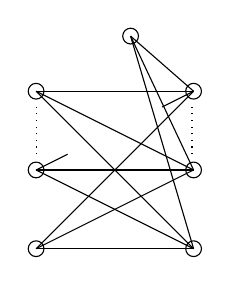
\begin{tikzpicture}
\draw (0.0, 0.0) circle (0.1cm);
\draw (0.0, 1.0) circle (0.1cm);
\draw (0.0, 2.0) circle (0.1cm);

\draw (2.0, 2.0) circle (0.1cm);
\draw (2.0, 0.0) circle (0.1cm);
\draw (2.0, 1.0) circle (0.1cm);
\draw (1.2, 2.7) circle (0.1cm);

\draw (0.0, 0.0) -- (2.0, 0.0);
\draw (0.0, 0.0) -- (2.0, 1.0);
\draw (0.0, 0.0) -- (2.0, 2.0);

\draw (0.0, 1.0) -- (2.0, 0.0);
\draw (0.0, 1.0) -- (2.0, 1.0);
\draw (0.0, 1.0) -- (0.4, 1.2);
\draw (1.6, 1.8) -- (2.0, 2.0);

\draw (0.0, 2.0) -- (2.0, 0.0);
\draw (0.0, 2.0) -- (2.0, 1.0);
\draw (0.0, 2.0) -- (2.0, 2.0);

\draw (1.2, 2.7) -- (2.0, 0.0);
\draw (1.2, 2.7) -- (2.0, 1.0);
\draw (1.2, 2.7) -- (2.0, 2.0);
\draw[dotted] (0.01, 1.2) -- (0.01, 1.8);
\draw[dotted] (1.98, 1.2) -- (1.98, 1.8);
\end{tikzpicture}
\end{center}
%
Back propagation for the ANN.
First define some shorthand:
\begin{equation} \label{eq:psi}
\psi^i_p = \sum_{k} y_k^i \omega_{p,k}^i + b^iu_p^i
\end{equation}
%
Then
\begin{equation} \label{eq:z}
z_p = g(\psi_p^n)
\end{equation}
%
and
%
\begin{equation} \label{eq:z}
y_p^{i+1} = g(\psi_p^i)
\end{equation}
%
define the error term
%
\begin{equation} \label{eq:error}
E = \frac{1}{2} \sum_k (z_k - t_k)^2
\end{equation}
%
then
%
\begin{equation} \label{eq:derror}
\frac{\partial E}{\partial z_p} = z_p - t_p
\end{equation}
%
at the last layer:
%
\begin{equation} \label{eq:last_layer_derror}
\frac{\partial E}{\partial \omega_{i,j}^n} =
\frac{\partial E}{\partial z_i} \frac{\partial z_i}{\partial \omega_{k_n, j}^n} =
\left ( z_i - t_i \right ) y_j^n g' (\psi_i^n) =
\frac{\partial E}{\partial \omega_{i,j}^n}
\end{equation}
%
\begin{equation} \label{eq:delta}
\delta_{i,j}^n = \frac{\partial E}{\partial \omega_{i,j}^n}
\end{equation}
%
expanding \ref{eq:delta} with \ref{eq:last_layer_derror}:
%
\begin{equation} \label{eq:delta_full}
\delta_{i,j}^n = 
\left ( z_i - t_i \right ) y_j^n g' (\psi_i^n)
\end{equation}
%
\begin{equation} \label{eq:gamma}
\gamma_{i,j}^{n+1} := (z_j - t_j) g'(\psi_j^n)
\end{equation}
%
then
%
\begin{equation} \label{eq:delta2}
\delta_{i,j}^{n-1} =
\sum_{k_{n+1}} \delta_{k_{n+1},j}^n \omega_{k_{n+1},i}^n
\end{equation}
%
and
%
\begin{equation} \label{eq:weights}
\omega_{new}^n = \omega_{old}^n - \eta \delta^n
\end{equation}
%
\end{document}
